% Oliver Erxleben, Martin Helmich
% Hardwarenahe System und Treiberprogrammierung
%
\documentclass[11pt]{scrartcl}

% own geometry
%\usepackage[a4paper, left=3cm, right=3cm]{geometry}

\usepackage[ngerman]{babel} 
\usepackage[utf8]{inputenc} 
\usepackage[T1]{fontenc}
\usepackage{graphicx}
\usepackage{color}
\usepackage{xcolor}
\usepackage{jurabib}
\usepackage{hyperref}
\usepackage{tikz}
\usepackage{booktabs}
\usepackage{enumitem}
\usepackage{here} % picture positioning


\renewcommand*{\jbauthorfont}{\textsc}
\renewcommand*{\bibfnfont}{\normalfont}
\renewcommand*{\biblnfont}{\textsc}
%\renewcommand*{\samepageibidemname}{Ebd.}
\renewcommand*{\bibbtsep}{In: }
\renewcommand*{\bibjtsep}{In: }
\renewcommand*{\bibpldelim}{(}
\renewcommand*{\biburlprefix}{}
\renewcommand*{\biburlsuffix}{}

\makeatletter
\renewcommand*{\jbshorttitlefont}{%
\ifthenelse{%
\equal{\jb@@type}{article}%
\or
\equal{\jb@@type}{periodical}%
\or
\equal{\jb@@type}{incollection}%
}{%
\upshape%
}{%
\textit%
}%
}
\makeatother

\renewcommand*{\bibprdelim}{)}
\renewcommand*{\ajtsep}{}
\renewcommand*{\bpubaddr} { :}
\renewcommand*{\jbbtasep} { ; }
\renewcommand*{\jbbfsasep} { ; }
\renewcommand*{\jbbstasep} { ; }
\renewcommand*{\bibbtasep} { ; }
\renewcommand*{\bibbfsasep} { ; }
\renewcommand*{\bibbstasep} { ; } %between second and third author sep
\renewcommand*{\jbbtesep} { ; } %between two editors sep
\renewcommand*{\jbbfsesep} { ; } %between first and second editor sep
\renewcommand*{\jbbstesep} { ; } %between second and third editor sep
\renewcommand*{\bibbtesep} { ; } %between two editors sep
\renewcommand*{\bibbfsesep} { ; } %between first and second editor sep
\renewcommand*{\bibbstesep} { ; } %between second and third editor sep
\AddTo\bibsgerman{\def\editorsname{(Hrsg.)}}
\AddTo\bibsgerman{\def\editorname{(Hrsg.)}}
%\jurabibsetup{super, citefull=first,ibidem}
%\jurabibsetup{ibidem}
%\jurabibsetup{authorformat=citationreversed}
%\jurabibsetup{authorformat=reducedifibidem}
\jurabibsetup{biblikecite}
%\jurabibsetup{bibformat=ibidem}
%\jurabibsetup{pages=always}
\jbfirstcitepageranges
\AddTo\bibsgerman{\def\herename{hier}}
\jbuseidemhrule

\jurabibsetup{
  authorformat={smallcaps,year,and,citationreversed},
  titleformat={colonsep,all,italic},
  commabeforerest,
  see,
  dotafter=bibentry,
  ibidem=strict,
  biblikecite
}

\renewcommand*{\bibbtasep}{ und } %
\renewcommand*{\bibbfsasep}{, }   %
\renewcommand*{\bibbstasep}{ und }
\renewcommand*{\jbtitlefont}{}
\renewcommand*{\bibtfont}{}
\renewcommand*{\bibbtfont}{}
\renewcommand*{\bibjtfont}{}
\renewcommand*{\bibapifont}{}
\renewcommand*{\jbshorttitlefont}{}



	%
	% CITATIONS
	%
\newcommand{\book}[2]{\footnote{\cite[Vgl.][#2]{#1}}}
\newcommand{\bookwf}[2]{\cite[Vgl.][#2]{#1}}
\newcommand{\bookdir}[2]{\footnote{\cite[][#2]{#1}}}
\newcommand{\inetwf}[1]{\cite[Vgl.][\citefield{url}{#1}]{#1}}
\newcommand{\inetwfdir}[1]{\cite[][\citefield{url}{#1}]{#1}}
\newcommand{\inet}[1]{\footnote{\inetwf{#1}}}
\newcommand{\inetdir}[1]{\footnote{\cite[][\citefield{url}{#1}]{#1}}}
\newcommand{\innerref}[1]{\footnote{Vgl. auch Kapitel \ref{#1} dieser Arbeit, S. \pageref{#1}}}
\newcommand{\vgl}[2]{\cite[Vgl.][#2]{#1}}
\newcommand{\citeauthoryear}[1]{\citeauthor{#1} (\citeyear{#1})}
\bibliographystyle{jurabib}

% setup of source code listings
\usepackage{listings}
\usepackage{caption}
\lstset{
	basicstyle=\footnotesize\ttfamily,	% default font
	numbers=left,						% line numbers placement
	numberstyle=\tiny,					% line numbers style
	%stepnumber=2,						% line number padding
	numbersep=5pt,						% padding between line numbers and code
	tabsize=2,							% 
	extendedchars=true,         
	breaklines=true,						% line breaks 
	keywordstyle=\color{red},
	frame=lrtb,
	stringstyle=\color{gray}\ttfamily,	% color of strings in code
	showspaces=false,					% visualize spaces
    showtabs=false,						% visualize tabs
    xleftmargin=17pt,
	framexleftmargin=17pt,
	framexrightmargin=5pt,
	framexbottommargin=4pt,
	showstringspaces=false				% visualize spaces in strings        
}

\lstset{
  literate={ö}{{\"o}}1
           {ä}{{\"a}}1
           {ü}{{\"u}}1
}
 
\lstloadlanguages{% Check docs for further languages ...
	C,
	C++,
	bash
}

% Directory Tree settings 
\makeatletter
\newcount\dirtree@lvl
\newcount\dirtree@plvl
\newcount\dirtree@clvl
\def\dirtree@growth{%
  \ifnum\tikznumberofcurrentchild=1\relax
  \global\advance\dirtree@plvl by 1
  \expandafter\xdef\csname dirtree@p@\the\dirtree@plvl\endcsname{\the\dirtree@lvl}
  \fi
  \global\advance\dirtree@lvl by 1\relax
  \dirtree@clvl=\dirtree@lvl
  \advance\dirtree@clvl by -\csname dirtree@p@\the\dirtree@plvl\endcsname
  \pgf@xa=0.5cm\relax
  \pgf@ya=-0.5cm\relax
  \pgf@ya=\dirtree@clvl\pgf@ya
  \pgftransformshift{\pgfqpoint{\the\pgf@xa}{\the\pgf@ya}}%
  \ifnum\tikznumberofcurrentchild=\tikznumberofchildren
  \global\advance\dirtree@plvl by -1
  \fi
}

\tikzset{
  dirtree/.style={
    growth function=\dirtree@growth,
    every node/.style={anchor=north},
    every child node/.style={anchor=west},
    edge from parent path={(\tikzparentnode\tikzparentanchor) |- (\tikzchildnode\tikzchildanchor)}
  }
}

\makeatother

\setlength{\parindent}{0pt}
\setlength{\parskip}\medskipamount

\tikzstyle{every node}=[font=\footnotesize]

%\DeclareCaptionFont{white}{\color{white}}
%\DeclareCaptionFormat{listing}{\colorbox{gray}{\parbox{\textwidth}{#1#2#3}}}
%\captionsetup[lstlisting]{format=listing,labelfont=white,textfont=white}

% layout the box
%\DeclareCaptionFormat{listing}{\colorbox[rgb]{0.43, 0.35, 0.35 {\parbox{\textwidth}{\hspace{15pt}#1#2#3}}}

% layout the caption ontop of code
%\captionsetup[lstlisting]{format=listing,labelfont=white,textfont=white, singlelinecheck=false, margin=0pt, font={bf,footnotesize}}

% Headings
\usepackage{fancyhdr}
\fancyhead[R]{}
\fancyfoot{}

% Document begins now
\begin{document}

\author{%
	Martin Helmich \small(\href{mailto:martin.helmich@hs-osnabrueck.de}{martin.helmich@hs-osnabrueck.de})\\%
	Oliver Erxleben \small(\href{mailto:oliver.erxleben@hs-osnabrueck.de}{oliver.erxleben@hs-osnabrueck.de})\\ \\%
	%
	Hochschule Osnabr"uck \\%
	Ingenieurswissenschaften und Informatik \\%
	Informatik - Mobile und Verteilte Anwendungen }

\title{
\includegraphics[scale=0.75,keepaspectratio]{images/hs_os.png}\linebreak \linebreak Entwicklung eines Treibers und einer Toolchain zur Administration eines Embedded Systems}
\subtitle{Am Beispiel einer ZPU unter Linux}

\maketitle
\thispagestyle{empty}
\pagebreak
\tableofcontents
\thispagestyle{empty}
\listoffigures

\lstlistoflistings

\thispagestyle{empty}
\pagebreak
\thispagestyle{empty}
\begin{abstract}
\textbf{Zusammenfassung:}\\ 	
Die vorliegende Arbeit wurde mit LaTeX verfasst und ist eine gemeinsame Arbeit von Oliver Erxleben und Martin Helmich für das Modul \textit{Hardwarenahe System- und Treiberprogrammierung} aus dem Master-Studiengang \textit{Informatik - Verteilte und Mobile Anwendungen} im Wintersemester 2012/13 an der Hochschule Osnabrück / University of Applied Sciences.

Das Thema der Arbeit lautet \textit{Entwicklung eines Treibers und einer Toolchain zur Administration eines Embedded Systems}. Im Kern beschreibt die Arbeit die Entwicklung eines Treibers für ein eingebettetes System unter Linux. Treiberprogrammierung unter anderen Systemen, wie zum Beispiel Microsoft Windows oder Apple Mac OS werden nicht betrachtet. Genauer wird zum einen ein Linux-Treiber für eine ZPU vorgestellt. Zum anderen werden Bibliotheken und Werkzeuge zur Verwendung in Anwenderprogrammen und zur Steuerung der ZPU beschrieben.
\\
Im ersten Teil der Arbeit wird das Konzept der Hardware und das Konzept des Treibers und der Programmierbibliotheken vorgestellt. In den darauffolgenden Abschnitten werden detailliert die einzelnen Komponenten des Treibers beschrieben. Anwenderprogramme zum Testen werden an geeigneten Stellen vorgestellt, bzw. auf das zugehörige Kapitel verwiesen.
\\
Sofern nicht anders angegeben, wird zum Kompilieren des Quellcodes der GNU-Compiler GCC unter Linux (Kernel-Version 2.6.XX) verwendet. 
\end{abstract}

\pagebreak
% set new page style

\pagestyle{fancy}
\setcounter{page}{1} 

\section{Einleitung}

% TODO: überarbeiten / erweitern
Täglich verwendet und verlässt sich unsere Gesellschaft auf computergestützte Anwendungen. Wir suchen, schreiben, drucken, kopieren, erstellen oder entfernen Daten. Nur allzu oft werden dabei Geräte verwendet, die Funktionen für den Anwender bereitstellen, oder aber das Funktionsspektrum des Comutersystems erweitern. Funktionen der Computerkomponenten werden durch Anwenderprogramme durchgeführt, die von einem Betriebssystem verwaltet werden. Das Betriebssystem verwaltet auch alle Komponenten des Computersystems. Diese Komponenten sind Software oder auch Hardware. Erst die Teamarbeit zwischen Hardware und Software ermöglicht für den Anwender die Ausführung komplexer Programme.

Das Betriebssystem steuert den Zugriff auf Hardware und benötigt Kenntnisse über die installierten Hardwarekomponenten. Das \textit{Wissen} über angeschlossene Hardwarekomponenten ist in sog. Gerätetreibern\footnote{Gerätetreiber: Softwaremodul, welches Zugriffe und Interaktionen mit installierter Hardware steuert.} hinterlegt. Es stellt einen Teil des Betriebssystemkerns dar, der für den Zugriff auf Hardware verantwortlich ist. Für jedes Gerät wird ein eigener Treiber benötigt. \footnote{(Vgl. \cite{ltp_book}, Kapitel 1)}

Die Entwicklung eines Gerätetreibers und zugehörige Softwarekomponenten stellen einen interessanten, wenn nicht sogar erstrebenswerten, Teil der Programmierung von Computersystemen dar.

\pagebreak

\section{Architektur}
 
\subsection{ZPU}


Der ZPU ist nach Angaben des Herstellers, Zylin AS, der kleinste 32-Bit-Mikroprozessor der Welt und zählt zu der Kategorie der \textit{Soft CPU}\footnote{Soft-CPU:}s. Die grundlegende Idee, bzw. Aufgabe einer Soft-CPU, bzw. der ZPU ist so wenig FPGA\footnote{FPGA: Field Programmable Gate Array}-Speicher wie möglich aufzunehmen und Berechnungen dem HDL\footnote{HDL: Hardware Description Language}-Programm zu überlassen.

Zur Programmierung der ZPU kann die GCC-Toolchain verwendet werden. Neben \textit{GDB} werden \textit{newlib} und \textit{libstdc+} unterstützt.

Weiterhin ist es möglich den ZPU mit einem eingebetteten Betriebssystem zu betreiben. Das \textit{eCos}\footnote{eCos:}-Embbedded Operating System wird vom ZPU unterstützt. 

% TODO: PCI Board Beschreibung überarbeiten
Neben dem ZPU sind weitere Komponenten auf dem PCI-Board enthalten. Zum einen zwei Ein- und Ausgabe-Fifos, welche zum Laden des Programms für die ZPU genutzt werden und zum anderen eine 7-Segment-Anzeige.

% TODO: überarbeiten
Die Hardware-Architektur der ZPU lässt sich in Abbildung \ref{zpu_architecture} veranschaulichen. 
Die Ein- und Ausgabe von Daten lassen sich über das Sende- und Empfangs-Fifo steuern. Zu beachten ist an dieser Stelle das die Fifos nach dem Ausgangspunkt (ZPU oder Linux-Kernel) zum Empfangen oder Senden genutzt werden. Aus Sicht der ZPU werden Daten gesendet wenn diese im Empfangs-Fifo des Kernels geschrieben werden. Empfangen werden Daten vom Kernel wenn diese in das Sende-Fifo geschrieben werden. 

\begin{figure}[H]
	\begin{center}
		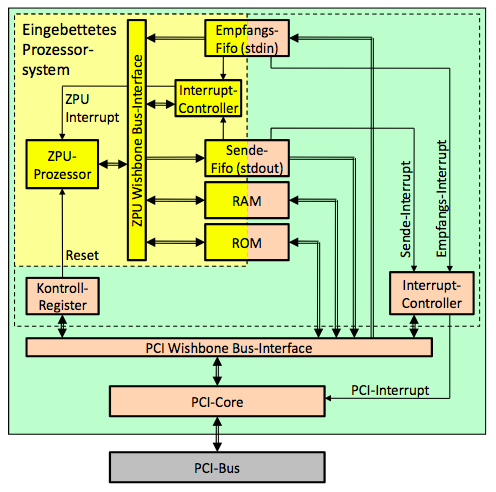
\includegraphics[width=0.9\textwidth]{images/zpu_architecture}
		\caption{Architektur der ZPU}
		\label{zpu_architecture}	
	\end{center}
\end{figure}

\subsection{Überblick über die Treiber-Toolchain}
Wie in der Einleitung bereits beschrieben, sollen neben dem Treiber-Modul auch Bibliotheken für Benutzerprogramme, sowie Benutzerprogramme selbst entwickelt werden. Die Abbildung \ref{zpu_overview} zeigt die drei Ebenen die entwickelt werden.

\begin{figure}[!htb]
	\begin{center}
		\begin{tikzpicture}
	\usetikzlibrary{positioning}
	\tikzstyle{node}=[anchor=mid,text centered,minimum height=2em];
	\tikzstyle{app}=[draw,fill=green!50,rectangle]
	\tikzstyle{lib}=[draw,fill=yellow!50,rectangle]
	\tikzstyle{dri}=[draw,fill=red!50,rectangle]
				
	\draw [lib] (6,0.5) rectangle +(2,0.75) node [node,midway] {libzpu};
	\draw [lib] (4cm-2pt,0.5) rectangle +(2,0.75) node [node,midway] {libintelhex};
				
	\draw [dri] (-0.5,-0.5) rectangle +(8.5,-0.75) node [node,midway] {modzpu};
	\draw [app] (6,2) rectangle +(2,0.75) node [node,midway] {zpuio};
	\draw [app] (4cm-2pt,2) rectangle +(2,0.75) node [node,midway] {zpuload};
					
	\draw [dashed] (0,0) -- (8,0);
	\draw [->] (7,0.5) -- (7,-0.5);
	\draw [->] (7,2) -- (7,1.25);
	\draw [->] (5,2) -- (5,1.25);
	\draw [->] (5.5,2) -- (6.5,1.25);
				
	\node [anchor=west] at (-0.5, 2.375) {Userspace-Programme};
	\node [anchor=west] at (-0.5, 0.875) {Bibliotheken};
\end{tikzpicture}
		\caption{Überblick ZPU-Toolchain}
		\label{zpu_overview}	
	\end{center}
\end{figure}

\pagebreak
\section{Linux-Treiber-Modul: modzpu}
% TODO: verfassen
Der Treiber für das Embedded System stellt die zentrale Steuerungssoftware für Host und für Treiber dar. Dieser Abschnitt gibt einen Überblick über das Treibermodul und stellt die wichtigsten Funktionen im Modul vor. Zur Übersichtlichkeit wurden Funktionen für den PCI-Treiber in mehrere Dateien aufgesplittet. Das Treibermodul ist wie folgt aufgebaut:

\begin{figure}[H]
\begin{center}
\frame{\begin{tikzpicture}[dirtree]
\node{module} 
    child { node {scripts}
            child { node {load.sh} }
            child { node {unload.sh} }
    }
    child { node {zpu\_commands.h} }
    child { node {modzpu.h} }
    child { node {modzpu.c} }
    child { node {fifo.c} }
    child { node {zpu\_io.c} }
    child { node {zpu\_irq.c} }
    child { node {zpu\_mem.c} }
    child { node {zpu\_open.c} }
    child { node {Makefile} }
    
    ; % finish nodes

\end{tikzpicture}}
\end{center}
\caption{Dateien des ZPU-Kernelmoduls.}
\end{figure}


\subsection{Installation}

Das Treibermodul lässt sich einfach über ein Makefile installieren, bzw. deinstallieren. Es befindet sich im Wurzelverzeichnis des Treibermoduls und benötigt die sich im Unterverzeichnis  \textit{scripts} befindenen Bash-Skripte \textit{load.sh} und \textit{unload.sh}. Die Bash-Skripte sind für das Laden und Entladen des Treibermoduls aus dem Kernel verantwortlich.
Das Listing \ref{modzpu_install} zeigt die bequeme Installation des Treibers. Anzumerken ist, dass der Eingriff in den Kernel und das Laden/Entladen des Moduls in den Kernel, bzw. aus dem Kernel, root-Rechte am Sytem benötigt. Äquivalent zum Listing \ref{modzpu_install} kann das Modul mittels \texttt{make uninstall} wieder entladen werden. 

\begin{lstlisting}[label=modzpu_install,language=bash, caption=Installation des Treibermoduls][!h]
> cd to/the/module/folder
> su # optional, if not root
> make
> make install
\end{lstlisting}

% TODO load unload skript beschreiben?!

\subsection{Initialisieren des Moduls}

Die Initialisierungsfunktion ist in der \textit{modzpu.h} deklariert und in der \textit{modzpu.c} implementiert. Das Listing \ref{modzpu_initfunc} zeigt die Implementierung der \textit{init}-Funktion.

\begin{lstlisting}[language=C, firstnumber=67, label=modzpu_initfunc, caption=modzpu Init-Funktion][h!]
static int __init init(void)
{
	int r;
	struct pci_driver *d = &(mypci_driver);

	d->name     = "zpu";
	d->id_table = (const struct pci_device_id*) &(id_table);
	d->probe    = mypci_probe;
	d->remove   = mypci_remove;

	if ((r = pci_register_driver(d)) != 0)
	{
		OUT_WARN("Could not register ZPU device driver.\n");
		return r;
	}

	OUT_DBG("Initialized module.\n");

	return 0;
}
\end{lstlisting}

Benötige Treiberinformationen werden in der Struktur \textit{mypci\_driver} gehalten. Die Struktur ist in \textit{linux/pci.h} deklariert und wird zur Registrierung der PCI-Hardware im Kernel benötigt (Vgl. siehe \cite{script_hwstp}, Seite 253).
 
Zur Fehlersicherung wird der Rückgabewert der Funktion \texttt{pci\_register\_driver(d)} überprüft und ggf. wird der Wert, sollte er nicht 0 sein, zurückgeliefert. 

Ausgaben erscheinen nur, wenn das DEBUG-Flag (siehe \textit{modzpu.h}) gesetzt ist. 
\subsection{Modul-Cleanup}
% TODO: ausbauen, pci_unregister_driver beschreiben?!
Die Struktur \texttt{\&mypci\_driver} wird der Kernelfunktion \textit{pci\_unregister\_driver} übergeben um das Modul aus dem Kernel zu entladen. 

\begin{lstlisting}[language=C, firstnumber=67, label=modzpu_cleanupfunc, caption=modzpu Cleanup-Funktion][h!]
void __exit cleanup(void)
{
	pci_unregister_driver(&mypci_driver);
	OUT_DBG("Unregistered PCI driver.\n");
}
\end{lstlisting}

\subsection{Speicher Mapping}

\begin{lstlisting}[language=C, firstnumber=67, label=modzpu_cleanupfunc, caption=modzpu Cleanup-Funktion][h!]

\end{lstlisting}

\subsection{IOCTRL}


\subsection{Lese- und Schreibzugriffe}

\begin{figure}[H]
	\begin{center}
		%include from external
		\begin{tikzpicture}
	\usetikzlibrary{positioning}
	\tikzstyle{pci}=[draw,fill=green!50,rectangle]
	\tikzstyle{krn}=[draw,fill=yellow!50,rectangle]
				
	\draw [fill=green!20] (0,-0.5) rectangle +(8,2.5);
	\draw [fill=yellow!20] (0,2.5) rectangle +(8,2.5);
				
	%\draw [<->] (1.8,0.9) -- (5,0.9);
	%\draw [<->] (3.8,1.1) -- (5,1.1);
	\draw [<->,dotted] (6,1.5) -- (6,3);
			
	\draw [<->,dotted] (1,0.2) -- (1,-0.2) -- (6.1,-0.2) -- (6.1,0.5);
	\draw [<->,dotted] (3,0.2) -- (3,-0) -- (5.9,0) -- (5.9,0.5);
				
	\draw [<->,dotted] (3.2,4.3) -- (3.2,4.5) -- (5.9,4.5) -- (5.9,4);
	\draw [<->,dotted] (1.2,4.3) -- (1.2,4.7) -- (6.1,4.7) -- (6.1,4);
				
	%\draw [<->] (1.8,3.4) -- (5,3.4);
	%\draw [<->] (3.8,3.6) -- (5,3.6);
				
	\node [anchor=north east] at (8,-0.5) {PCI-Hardware};
	\node [anchor=south east] at (8, 5.0) {Kernel};
				
	\draw [pci] (0.2,0.2) rectangle +(1.6,1.6) node [align=left,midway] {Eingabe-\\FIFO\\(\texttt{stdin})};
	\draw [pci] (2.2,0.2) rectangle +(1.6,1.6) node [midway,align=left] {Ausgabe-\\FIFO\\(\texttt{stdout})};
					
	\draw [krn] (0.2,2.7) rectangle +(1.6,1.6) node [midway,align=left] {Eingabe-\\FIFO};
	\draw [krn] (2.2,2.7) rectangle +(1.6,1.6) node [midway,align=left] {Ausgabe-\\FIFO};
				
	\draw [->] (1,2.7) -- (1,1.8);
	\draw [<-] (3,2.7) -- (3,1.8);
				
	\draw [->] (1,5.5) -- (1,4.3);
	\draw [<-] (3,5.5) -- (3,4.3);
	\node [anchor=south] at (3,5.5) {\texttt{read()}};
	\node [anchor=south] at (1,5.5) {\texttt{write()}};
				
	\draw [pci] (5,0.5) rectangle +(2,1) node [align=left,midway] {Interrupt-\\Controller};
		\draw [krn] (5,3) rectangle +(2,1) node [midway] {IRQ-Handler};
\end{tikzpicture}
		\caption{ZPU-Ein und Ausgabe}
		\label{zpu_io}
	\end{center}
\end{figure}

Die Lese - und Schreibzugriffe auf, bzw. von der ZPU, sind in Abbildung \ref{zpu_io} veranschaulicht. Das Treibernmodul kann aus dem Kernel Daten über das Eingabe-FIFO schreiben und über das Ausgabe-FIFO Daten von der PCI-Hardware holen.

\begin{lstlisting}[language=C, firstnumber=14, label=modzpu_mychr_write, caption=ZPU-Schreib-Funktion][h!]
static ssize_t mychr_write (struct file *filep, const char __user *data, size_t count, loff_t *offset)
{
	fifo_t			*f	= &(zpu_io_stdin);
	unsigned int	n;
	
	if (FIFO_FULL(f))
	{
		ZPU_ENABLE_STDIN_IR();
	
		if (filep->f_flags & O_NONBLOCK)
		{
			return -EAGAIN;
		}
		else if (wait_event_interruptible(f->queue, FIFO_NOT_FULL(f)) != 0)
		{
			return -EINTR;
		}
	}
	
	n = count < FIFO_FREE(f) ? count : FIFO_FREE(f);
	
	if (f->write + n <= f->size)
	{
		if (copy_from_user(f->data + f->write, data, n) > 0) return -EAGAIN;
		f->write = (f->write + n) % f->size;
	}
	else
	{
		unsigned int size1 = (f->size - f->write);
		unsigned int size2 = (n - size1);
		
		if (copy_from_user(f->data + f->write, data, size1) +
		    copy_from_user(f->data, data + size1, size2) > 0) return -EAGAIN;
		
		f->write = size2;
	}
	
	f->count = f->count + n;
	ZPU_ENABLE_STDIN_IR();
	
	return n;
}
\end{lstlisting}


\pagebreak
\section{Parsing der Intel HEX-Dateien: Die libcintelhex}
\label{chapter_libcintelhex}

Die Logik zum Parsen der Intel HEX-formatierten Eingabedateien wurde in eine eigene Programmbibliothek ausgegliedert. Der folgende Abschnitt beschreibt zunächst das Intel HEX-Datenformat, erläutert anschließend Installation und Schnittstellen der (im Rahmen dieser Arbeit entstandenen) cintelhex-Bibliothek und erklärt die dort verwendeten Algorithmen.

\subsection{Das Intel HEX-Format}

Bei dem \emph{INTEL Hexadecimal Object File Format} (kurz \emph{INTEL HEX}) handelt es sich um ein Dateiformat zur Codierung binärer Daten in ASCII-Dateien. Ursprünglich ausgelegt für 8-Bit-Intelprozessoren mit Adressräumen von 16 Bit, wurde das Format später erweitert für 16-Bit-Prozessoren mit 20-Bit-Adressräumen und für 32-Bit-Prozessoren.
\footnote{Vgl. \cite[S. 4]{intelhex}}

Der Aufbau eines Intel HEX-Datensatzes ist in Abbildung \ref{record_structure} dargestellt. Jeder Datensatz beginnt mit einem \emph{Record Mark} (ein \texttt{:}-Zeichen, oder \texttt{0x3A} in ASCII). Es folgen die Länge des Datensatzes (1 Byte, codiert in 2 ASCII-Zeichen), der Adress-Offset (2 Byte), der Typ des Datensatzes (1 Byte), der eigentliche Datensatz (variabel, bis zu 255 Bytes) und eine Prüfsumme (1 Byte), anhand derer die Korrektheit des Datensatzes überprüft werden kann.

\begin{figure}[h!]
\begin{center}
\begin{tabular}{cccccc}
	\toprule
	\texttt{:} & \texttt{10} & \texttt{0400} & \texttt{00} & \texttt{B0B0B98B02D0B0B0B88800400000000} & \texttt{29} \\ \midrule
	& Länge & Adresse & Typ & Daten & Prüfsumme \\ \bottomrule
\end{tabular}
\caption{Aufbau eines Intel HEX-Datensatzes}
\label{record_structure}
\end{center}
\end{figure}

Neben regulären Datensätzen (Typ \texttt{0x00}) und einem EOF-Datensatz (Typ \texttt{0x01}), der das Dateiende markiert, kennt die Spezifikation noch weitere Datensatz-Typen, die beispielsweise die Nutzung eines 20- oder 32-Bit-Adressraums ermöglichen. So kann beispielsweise ein spezieller \emph{Extended Linear Address Record} (Typ \texttt{0x04}) verwendet werden, um durch Angabe einer \emph{Upper Linear Base Address} den Adressraum auf 32 Bit zu erweitern.

Da der Speicher des verwendeten ZPU-Boards nur 8 KiB umfasst, ist eine Verwendung der 32-Bit-Funktionen nicht notwendig (16 Bit adressieren maximal $2^{16} = 64$ KiB). Aus diesem Grund bietet die cintelhex-Bibliothek nur experimentelle Unterstützung für 32-Bit-Adressen.

\begin{lstlisting}[caption=Beispiel einer Intel HEX-Eingabedatei]
:1000000000000000000000000000000000000000F0
:0400100000000000EC
:100400000B0B0B98B02D0B0B0B8880040000000029
:1004100000000000000000000000000000000000DC
// ...
:1010E200000008D9000008D9000008D9000008D97A
:1010F200000008D9000008D9000008D9000008D96A
:0C110200000008D9000008D9000008D93E
:0400000300000400F5
:00000001FF
\end{lstlisting}

\subsection{Installation}

Die Installation der cintelhex-Bibliothek erfolgt mit den Unix-üblichen \texttt{configure}- und \texttt{make}-Befehlen. Außer dem Build-Tool \texttt{make}, der C-Standardbibliothek und dem GCC werden keine Abhängigkeiten benötigt.

\begin{lstlisting}[caption=Installation der cintelhex-Bibliothek]
> ./configure # optional: --prefix=/usr/local
> make
> make install
> ldconfig
\end{lstlisting}

Bei der Installation wird die Datei \texttt{libcintelhex.so} nach \texttt{<prefix>/lib}, und die Datei \texttt{cintelhex.h} nach \texttt{<prefix>/include} installiert. Das Standardpräfix ist \texttt{/usr/local}.

Bei Verwendung des Standardpräfix kann die cintelhex-Bibliothek beim Linken durch den GCC-Parameter \texttt{-l cintelhex} aktiviert werden.

\subsection{Schnittstellenbeschreibung}

Die Methoden der cintelhex-Bibliothek können durch inkludieren der Header-Datei \texttt{cintelhex.h} verwendet werden. In der Datei werden folgende wichtigen Methoden deklariert:

\begin{description}[style=unboxed]
	\item[ihex\_recordset\_t* ihex\_rs\_from\_file(char* filename)] Diese Methode liest den Inhalt einer Intel HEX-Datei (der Dateiname wird durch \texttt{filename} beschrieben) in eine \texttt{ihex\_recordset\_t}-Struktur (siehe auch Abschnitt \ref{ihex_structs}). Sie liefert einen Zeiger auf die ausgelesene Struktur zurück, oder \texttt{NULL} im Fehlerfall.
	\item[ihex\_recordset\_t* ihex\_rs\_from\_string(char* data)] Diese Methode verhält sich genau wie \texttt{ihex\_rs\_from\_file}, erwartet als Eingabeparameter jedoch direkt einen Zeiger auf einen Intel HEX-String.
	\item[int ihex\_mem\_copy(ihex\_recordset\_t *rs, void* dst, ulong\_t n, ihex\_width\_t w, ihex\_byteorder\_t o)] Diese Methode kopiert das durch eine Intel HEX-Datei beschriebene Programm an eine beliebige Stelle im Speicher. Das zu ladende Programm wird durch die Struktur \texttt{rs} beschrieben. Der Zeiger \texttt{dst} beschreibt die Zielposition im Speicher (dies kann auch ein durch \texttt{mmap} abgebildeter Gerätespeicher sein). \texttt{n} beschreibt die Größe des Zielbereichs. Die Methode liefert im Erfolgsfall 0, ansonsten einen Fehlercode zurück.
	\item[char* ihex\_error()] Diese Methode liefert eine Beschreibung des zuletzt aufgetretenen Fehlers zurück. Falls kein Fehler aufgetreten ist, wird \texttt{NULL} zurückgeliefert.
	\item[ihex\_error\_t ihex\_errno()] Diese Methode liefert den Fehlercode des zuletzt aufgetretenen Fehlers zurück. Falls kein Fehler aufgetreten ist, wird \texttt{0} zurückgeliefert.
\end{description}

\subsection{Datenstrukturen}
\label{ihex_structs}

Die cintelhex-Bibliothek definiert die beiden Datenstrukturen \texttt{ihex\_recordset\_t} und \texttt{ihex\_record\_t}. Sie sind wie folgt definiert:

\begin{lstlisting}[language=C,morekeywords={uint\_t, ihex\_rtype\_t, ihex\_addr\_t, ihex\_rdata\_t, ihex\_rchks\_t, ihex\_record\_t, ihex\_recordset\_t}, caption=Definition der \texttt{ihex\_record\_t}- und \texttt{ihex\_recordset\_t}-Strukturen]
/// Models a single Intel HEX record.
typedef struct ihex_record {
	uint_t       ihr_length;   //!< Length of the record in bytes.
	ihex_rtype_t ihr_type;     //!< Record type (see ihex_rtype_t).
	ihex_addr_t  ihr_address;  //!< Base address offset.
	ihex_rdata_t ihr_data;     //!< Record data.
	ihex_rchks_t ihr_checksum; //!< The record's checksum.
} ihex_record_t;

/// Models a set of Intel HEX records.
typedef struct ihex_recordset {
	uint_t         ihrs_count;   //!< Amount of records.
	ihex_record_t *ihrs_records; //!< A list of record (with ihrs_count elements).
} ihex_recordset_t;
\end{lstlisting}

Abbildung \ref{lcih_datastructs} zeigt zudem die Beziehungen der Datenstrukturen untereinander. Das Attribut \texttt{ihex\_data} der Struktur \texttt{ihex\_record\_t} ist ein Zeiger auf ein \texttt{uint8\_t}-Feld der Länge \texttt{ihr\_length}.

\begin{figure}[!htb]
	%include from externl
	\begin{center}
		\begin{tikzpicture}
	\usetikzlibrary{arrows}
	\tikzstyle{attr}=[midway,text width=3.3cm,text height=0.3cm]
	\tikzstyle{green}=[fill=green!20]
	\tikzstyle{yellow}=[fill=yellow!20]	
			
	\draw [fill=green!50] (0,0) rectangle +(3.5,0.5) node [attr] {\texttt{ihex\_recordset\_t}};
	\draw [green] (0,-0.5) rectangle +(3.5,0.5) node [attr] {\texttt{ihrs\_count} = 2};
	\draw [green] (0,-1) rectangle +(3.5,0.5) node [attr] {\texttt{ihrs\_records} = };
			
	\draw [fill=yellow!50] (0,-2) rectangle +(3.5,0.5) node [attr] {\texttt{ihex\_record\_t}};
	\draw [yellow] (0,-2.5) rectangle +(3.5,0.5) node [attr] {\texttt{ihr\_length} = 4};
	\draw [yellow] (0,-3) rectangle +(3.5,0.5) node [attr] {\texttt{ihex\_type} = 0x00};
	\draw [yellow] (0,-3.5) rectangle +(3.5,0.5) node [attr] {\texttt{ihex\_addr} = 0x00};
	\draw [yellow] (0,-4) rectangle +(3.5,0.5) node [attr] {\texttt{ihex\_data} = };
			
	\draw [fill=yellow!50] (3.5,-2) rectangle +(3.5,0.5) node [attr] {\texttt{ihex\_record\_t}};
	\draw [yellow] (3.5,-2.5) rectangle +(3.5,0.5) node [attr] {\texttt{ihr\_length} = 6};
	\draw [yellow] (3.5,-3) rectangle +(3.5,0.5) node [attr] {\texttt{ihex\_type} = 0x00};
	\draw [yellow] (3.5,-3.5) rectangle +(3.5,0.5) node [attr] {\texttt{ihex\_addr} = 0x04};
	\draw [yellow] (3.5,-4) rectangle +(3.5,0.5) node [attr] {\texttt{ihex\_data} = };
			
	\draw[*->] (3,-0.7) -- (3,-1.5);
	\draw[*->] (2.5,-3.7) -- (2.5,-4.5) -- (0.75/2, -4.5) -- (0.75/2,-5);
	\draw[*->] (6,-3.7) -- (6,-4.5) -- (3.5+0.75/2, -4.5) -- (3.5+0.75/2,-5);
			
	\foreach \x in {0,0.75,1.5,2.25}{
		\draw (\x, -5.5) rectangle +(0.75,0.5) node [attr,text width=0.7cm] {0x00};
	};
			
	\foreach \x in {3.5,4.25,5,5.75,6.5,7.25}{
		\draw (\x, -5.5) rectangle +(0.75,0.5) node [attr,text width=0.7cm] {0x00};
	};
\end{tikzpicture}
	\end{center}
	\caption{Datenstrukturen der libcintelhex}
	\label{lcih_datastructs}
\end{figure}

\subsection{Fehlercodes}

Die \texttt{cintelhex.h} definiert die folgenden Fehlerkonstanten:

\begin{description}
	\item[IHEX\_ERR\_INCORRECT\_CHECKSUM] Tritt auf, wenn die Prüfsumme eines Eintrages ungültig ist. Zur Verifizierung der Prüfsumme werden alle Bytes eines Eintrages (einschließlich der Prüfsumme selbst) aufsummiert. Ist das unterste Byte der Summe $=0$, ist die Prüfsumme korrekt.
	\item[IHEX\_ERR\_NO\_EOF] Tritt auf, wenn die Eingabedatei keinen EOF-Eintrag (Typ \texttt{0x01}) enthält.
	\item[IHEX\_ERR\_PARSE\_ERROR] Tritt auf, wenn die Eingabedatei ungültig formatiert ist (etwa bei Fehlen des Record Marks (\texttt{:})).
	\item[IHEX\_ERR\_WRONG\_RECORD\_LENGTH] Tritt auf, wenn die tatsächliche Länge eines Datensatzes nicht der im ersten Byte angegebenen entspricht.
	\item[IHEX\_ERR\_NO\_INPUT] Tritt auf, wenn die Eingabedatei nicht existiert, oder nicht geöffnet werden konnte.
	\item[IHEX\_ERR\_UNKNOWN\_RECORD\_TYPE] Tritt auf, wenn ein Datensatz eine ungültige Typ-Bezeichnung (Byte 4) hat).
	\item[IHEX\_ERR\_PREMATURE\_EOF] Tritt auf, wenn der EOF-Datensatz (Typ \texttt{0x01}) in einer anderen Zeile als der letzten auftritt.
	\item[IHEX\_ERR\_ADDRESS\_OUT\_OF\_RANGE] Tritt auf, wenn an eine ungültige Adresse geschrieben werden soll.
	\item[IHEX\_ERR\_MMAP\_FAILED] Tritt auf, wenn eine Eingabedatei nicht in den Speicher gemappt werden konnte.
\end{description}

\subsection{Anwendungsbeispiel}

Listing \ref{cintelhex-example} zeigt ein einfaches Anwendungsbeispiel der cintelhex-Bibliothek. Der Einfachheit halber zeigt die Variable \texttt{d} hier nur auf einen dynamisch alloziierten Speicherbereich, könnte jedoch auch ebenso gut auf den per \texttt{mmap} abgebildeten Speicher des ZPU-Boards zeigen.

\begin{lstlisting}[language=C,caption=Anwendungsbeispiel der cintelhex-Bibliothek,label=cintelhex-example]
#include <stdlib.h>
#include <cintelhex.h>

int main()
{
	ihex_recordset_t* r = ihex_rs_from_file("input.hex");
	void*             d = malloc(8192);
	
	if (r != NULL)
	{
		return ihex_mem_copy(r, d, 8192, IHEX_WIDTH_32BIT, IHEX_ORDER_BIGENDIAN);
	}
	return ihex_errno();
}
\end{lstlisting}

\subsection{Besonderheiten der Umsetzung}

%\subsubsection{8- vs. 32-Bit-Zugriff}

Erste Versionen der cintelhex-Bibliothek versuchten, den Zielspeicherbereits byteweise zu befüllen. Während dies bei Tests an dynamisch alloziiertem RAM kein Problem darstellte, wurde schnell deutlich, dass diese Art des Zugriffs bei dem Speicher des ZPU-Boards nicht funktioniert. Listings \ref{zpu_mem_8bit} und \ref{zpu_mem_32bit} verdeutlichen das Problem.

\begin{lstlisting}[float=p,language=C,caption=Unerwartetes Verhalten des ZPU-Speichers bei 8-Bit-Zugriff,morekeywords={uint8_t,uint32_t},label=zpu_mem_8bit]
uint8_t *d; // d zeigt auf den gemappten Geraetespeicher

d[0x00] = 0x0b;
printf("%02x \n", d[0x00]); // Gibt "0b" aus (korrekt).

d[0x01] = 0x98;
printf("%02x \n", d[0x00]); // Gibt "00" aus (sollte immer noch "0b" sein)!
printf("%02x \n", d[0x01]); // Gibt "98" aus (korrekt).
\end{lstlisting}

\begin{lstlisting}[float=p,language=C,caption=Korrektes Verhalten des ZPU-Speichers bei 32-Bit-Zugriff,morekeywords={uint8_t,uint32_t},label=zpu_mem_32bit]
uint8_t *d; // d zeigt auf den gemappten Geraetespeicher

*((uint32_t*) d) = 0x0000980b;

printf("%02x \n", d[0x00]); // Gibt "0b" aus (korrekt).
printf("%02x \n", d[0x01]); // Gibt "98" aus (korrekt).
\end{lstlisting}

Weiterhin fiel auf, dass das geladene Programm von der ZPU nur dann korrekt ausgeführt werden konnte, wenn die Intel HEX-Daten als 32-Bit-Blöcke in \emph{Big Endian}-Reihenfolge interpretiert wurden. Abbildung  \ref{zpu_addresses} verdeutlicht diesen Zusammenhang.

Die cintelhex-Bibliothek berücksichtigt diesen Zusammenhang. So akzeptiert die Methode \texttt{ihex\_mem\_copy} einen Parameter \texttt{w}, über welchen die Wortbreite angegeben werden kann, sowie einen Parameter \texttt{o}, welcher die Byte-Reihenfolge beschreibt. Listing \ref{ihex_copy_algo} beschreibt den Algorithmus zum Laden eines Intel HEX-Datensatzes in den ZPU-Speicher.

\begin{figure}
\begin{center}
\begin{tabular}{lrrrrrrrrc}
	\toprule
	Daten   &  0B &  0B &  0B &  98 &  B0 &  2D &  0B &  0B & $\ldots$ \\ \midrule
	Adresse & 403 & 402 & 401 & 400 & 407 & 406 & 405 & 404 & $\ldots$ \\ \bottomrule
\end{tabular}
\end{center}
\caption{Übersetzung von Binärdaten in lauffähige ZPU-Programme.}
\label{zpu_addresses}
\end{figure}

\begin{lstlisting}[float=p,language=C,caption=Algorithmus zum Laden eines Intel HEX-Datensatzes in den ZPU-Speicher,morekeywords={uint8_t, uint32_t, ihex_width_t, ihex_record_t, ihex_byteorder_t},label=ihex_copy_algo]
ihex_width_t     w = IHEX_WIDTH_32BIT;     //<! Wortbreite in Byte
ihex_byteorder_t o = IHEX_ORDER_BIGENDIAN; //<! Byte-Reihenfolge
uint8_t          j, l;                     //<! Laufvariablen
ihex_record_t   *x;                        //<! Ein IHEX-Datensatz

for (j = 0; j < x->ihr_length; j += w)
{
	uint32_t  v      = 0;
	uint32_t *target = (uint32_t*) (d + address + j);
					
	for (l = 0; (l < w) && (j + l < x->ihr_length); l ++)
	{
		v += x->ihr_data[j+l] << (8 * ((o == IHEX_ORDER_BIGENDIAN) ? ((w - 1) - l) : l));
	}
	*(target) = v;
}
\end{lstlisting}

\pagebreak
\section{Programmierung der ZPU: Die libzpu}
\label{chapter_libzpu}

% TODO: erweitern
Die \textit{libzpu} stellt die für Anwenderprogramme benötigten Funktionen des Treibers zur Verfügung. Die Schnittstelle wurde zur Abstrahierung der Logik für Anwenderprogramme erstellt. Dieser Abschnitt beschreibt die Bibliotheksfunktionen und zeigt exemplarisch wie die Bibliothek in Anwenderprogrammen genutzt werden kann. 

Die Quelltexte für die Bibliothek finden sich auf dem beigelegten Datenträger oder aber auf Github: \url{https://github.com/olivererxleben/zpulib}. 

\subsection{Installation}
Um die Bibliothek auf einem Linux-System zu installieren muss in das Wurzelverzeichnis der Quellen gewechselt werden und dort über ein Unix-übliches Makefile ausgeführt werden.

\begin{lstlisting}[language=bash,caption=Installation der zpulib-Bibliothek]
# in directory
> ./configure
> make
> make install
\end{lstlisting}

\subsection{Typdefinitionen und Variablen}

Die zpulib verwendet zur Fehlerbehandlung und für Funktionsrückgaben zwei eigene Typen und zwei globale Variablen. Das Listing \ref{zpulib_types_vars} zeigt dessen Deklaration in der zpu.h.

\begin{lstlisting}[language=C,firstnumber=28,caption=zpulib Typen und Variblen,label=zpulib_types_vars]
// TYPE DEFINITIONS

typedef unsigned int uint_t;
typedef uint_t       zpu_error_t;

// GLOBAL VARIABLES

#ifdef ZPU_C
static zpu_error_t zpu_last_errno = 0;
static char*       zpu_last_error = NULL;
#else
extern zpu_error_t zpu_last_errno; //!< Error code of last error.
extern char*       zpu_last_error; //!< Description of last error.
#endif

\end{lstlisting}

\texttt{zpu\_error\_t} wird beispielsweise von 

\subsection{Schnittstellenbeschreibung}
Die Methoden der libzpu können durch das Inkludieren der \texttt{zpu.h} in ein Anwenderprogramm benutzt werden. Die \textit{zpulib} benutzt zudem Funktionen der \textit{libcintelhex} um Hex-Dateien zu laden. Nachfolgend werden die Funktionen der zpulib beschrieben.
%Desweiteren existiert die \texttt{zpu\_commands.h}, in der die IO-Kontrolle für die ZPU implementiert ist. 

\begin{description}[style=unboxed]
	\item[zpu\_error\_t zpu\_load\_from\_file(char* filename);] 
	Die Methode wird verwendet um eine neues Programm in die ZPU zu laden. Vor dem Laden des Programms wird die ZPU in in den sog. \textit{reset}-Modus gesetzt. Erst danach wird das zu ladene Programm von der Intel Hex Bibliothek geparsed und in den ROM der ZPU kopiert. Die Programm-Datei muss vom Typ INTEL Hex sein. 
	
	\item[int zpu\_stop();]
	Versetzt die ZPU in den \textit{reset}-Modus. Liefert \texttt{ZPU\_ERR\_OK} bei Erfolg zurück. Andernfalls einen Error Code. 
	
	\item[int zpu\_start();]
	Versetzt die ZPU aus denm \textit{reset}-Modus in den regulären Betriebszustand zurück. Die Methode liefert \texttt{ZPU\_ERR\_OK} bei Erfolg zurück. Andernfalls einen Error Code.
	
	\item[zpu\_error\_t zpu\_errno();]
	Eine Hilfsmethode zum Debuggen von Anwenderprogrammen. Sie liefert die Nummer des zuletzt aufgetretenen Fehlers zurück. 
	
	\item[char* zpu\_error();]
	Eine Hilfesmethode zum Debuggen von Anwenderprogrammen. Sie liefert den zuletzt aufgetretenen Fehler zurück. 
\end{description}

\subsection{Fehlercodes}
Neben Typen, Variablen und Funktionen definiert die zpulib auch Fehlercodes, welche beim Debugging von Anwenderprogrammen genutzt werden können.  
Folgende Fehlerkonstanten werden in der \texttt{zpu.h} deklariert:
% TODO: Beschreibungen hinzufügen
\begin{description}
    \item[\#define ZPU\_ERR\_OK              0x00]
    OK, bzw. 0, wird zurückgegeben wenn kein Fehler aufgetreten ist. 
    
    \item[\#define ZPU\_ERR\_PARSEERROR      0x01]
    Dieser Fehlercode wird von der zpulib zurückgegeben, wenn ein ZPU-Programm von der libchintelhex nicht analysiert werden konnte. 
    
    \item[\#define ZPU\_ERR\_DEVFILEOPEN     0x02]
    Der Fehlercode tritt auf wenn ein ZPU-Programm nicht geöffnet werden konnte. Zum Beispiel wenn die Datei nicht gefunden wurde. 
    
    \item[\#define ZPU\_ERR\_MMAP            0x03]
    Der MMAP-Fehlercode wird zurückgeliefert, wenn das Mapping der ZPU fehlgeschlagen ist. 
    
    \item[\#define ZPU\_ERR\_MEMCOPY         0x04]
    Bei dieser Fehlerkonstanten handelt es sich um den Fehler der beim Kopieren in den RAM der ZPU geschehen kann. 
    
    \item[\#define ZPU\_ERR\_COULDNOTSTOP    0x05]
    Der Fehler wird zurückgegeben wenn die ZPU nicht in den \textit{reset}-Modus versetzt werden konnte.
    
    \item[\#define ZPU\_ERR\_COULDNOTSTART   0x06]
    Wird zurückgegeben, wenn die ZPU nicht aus dem \textit{reset}-Modus zurück in den normalen Betriebszustand versetzt werden konnte. 
    
\end{description}

Azumerken ist, dass allle Fehlercodes in den Funktionsimplementierung Verwendung finden (siehe weitere Abschnitte). 

\subsection{Dateien laden} 

\subsection{ZPU Starten und Stoppen}

\pagebreak
\section{Anwenderprogramme}

Zur Steuerung des ZPU-Boards wurden schließlich die Werkzeuge \emph{zpuload}   und \emph{zpuio} entwickelt. Das Paket liegt dieser Arbeit auf Datenträger bei, und befindet sich im Verzeichnis \texttt{apps/zputools}.

\subsection{Installation}

\emph{zpuload} und \emph{zpuio} gehören beide zum \emph{zputools}-Paket, können also gemeinsam installiert werden. Wie bei den anderen im Rahmen dieser Arbeit entstandenen Pakete, reicht auch hier der übliche Dreizeiler zur Installation aus:

\begin{lstlisting}[caption=Installation der zputools-Werkzeuge]
> ./configure # optional mit --prefix=...
> make
> make install
\end{lstlisting}

Bei der Installation werden die ausführbaren Programme \emph{zpuload} und \emph{zpuio} (abhängig vom prefix) nach \texttt{/usr/local/bin} kopiert.

Die \emph{zputools} benötigen einen GCC, die C-Standardbibliothek, sowie eine installierte cintelhex-Bibliothek (siehe Abschnitt \ref{chapter_libcintelhex}) und eine installierte zpu-Bibliothek (siehe Abschnitt \ref{chapter_libzpu}). Das \emph{configure}-Skript überprüft diese Abhängigkeiten automatisch.

\subsection{Programme laden mit zpuload}

Das \emph{zpuload}-Programm verwendet die Funktionen der \emph{cintelhex}- und \emph{zpu}-Bibliotheken, um ein neues Programm in den ZPU-Prozessor zu laden.

Hierzu wird per \texttt{zpu\_load\_from\_file(file)}-Methode ein neues Programm in den RAM der ZPU geladen (diese Methode versetzt die ZPU zuvor implizit in des Reset-Modus und startet sie anschließend wieder).

\begin{lstlisting}[caption=Verwendung des zpuload-Werkzeugs]
> /usr/local/bin/zpuload input.hex
Loading program from "input.hex"...
Loaded program.
\end{lstlisting}

\subsection{Ein- und Ausgabe mit zpuio}

Das \emph{zpuio}-Werkzeug dient dazu, Ein- und Ausgaben an den ZPU-Prozessor zu übermitteln. Dieses Programm ist vor allem als interaktive Schnittstelle gedacht.

\begin{lstlisting}[caption=Verwendung des zpuio-Werkzeugs]
> /usr/local/bin/zpuio
output (11) > Hello World
input > abcd
output (4) > Abcd
input >
\end{lstlisting}

Neben der Verwendung des \emph{zpuio}-Werkzeugs kann auch direkt in/aus der Gerätedatei \emph{/dev/zpu} geschrieben und gelesen werden.

\pagebreak
\section{Fazit}

Mit den im Rahmen dieser Arbeit entwickelten Kernel-Module, Bibliotheken und Anwenderprogramme steht eine einfach benutzbare und gut erweiterbare Toolchain zur Arbeit mit einem ZPU-Board zur Verfügung.

Um die Arbeit mit diesen Werkzeugen weiter zu vereinfachen, wäre in einer fortführenden Arbeit beispielsweise möglich, über entsprechende udev-Regeln das Kernelmodul automatisch zu laden, die entsprechenden Gerätedateien zu erstellen. Zudem könnte über eine udev-Regel bereits beim Booten durch einen Aufruf des \textit{zpuload}-Programms eine initiale Firmware in die ZPU geladen werden.

Um die Upgrade-Fähigkeit des Kernel-Moduls über mehrere Kernel-Versionen hinweg sicherzustellen, böte sich zudem die Verwendung des von Dell entwickelten DKMS-Frameworks an.\footnote{Vgl. \cite{dkms-ljournal}.}

\pagebreak % content ends here

\fancyhead[R]{}

\thispagestyle{empty}

\renewcommand*{\biburlprefix}{(URL: }
\renewcommand*{\biburlsuffix}{)}

\pagebreak
\addcontentsline{toc}{section}{Literaturverzeichnis} % Eintrag ins Inhaltsverzeichnis
\bibliography{bib/bib}

\appendix

\end{document}
